\documentclass{article}
\usepackage{algorithm2e}
\usepackage[T1]{fontenc}
\setlength{\parindent}{0pt}
\setlength{\parskip}{0.5em}
\usepackage{graphicx}

\title{Project CME211 - Writeup}
\author{Paula Charles}
\date{December 2021}

\begin{document}

\maketitle

\section{Introduction}

In this project, we aim at solving 2D heat equations. To do 
so, we use sparse matrix solvers in C++. We use the finite-
difference method to discretize the system into a grid of 
points. We then solve this system using our matrix solvers 
and vizualize the results. This enables us to 
visualize heat maps of systems that are in contact with hot and 
cold streams, and for which the temperature is not uniform.

This solution is only able to solve simplified periodic systems.

\section{CG solver implementation}

To implement the CG solver, we use 2 classes:

\begin{itemize}
    \item The Class SparseMatrix that handles sparse matrices. 
    It initializes a matrix as a COO matrix, which can then be 
    modified thanks to its method AddEntry(). It has then some 
    more methods that can be used for our 2D heat problem: a 
    method that converts the COO matrix into a CSR matrix 
    (that is more efficient for calculations) and a 
    get\_CGSolver() method that uses the files CGSolver.hpp/cpp 
    to get a solution. A pseudo-code for this solver is available below.
    
    To implement the Conjugate gradient code, we used several 
    functions to prevent redundancy. These functions can be found
    in the matvecops.cpp file and enable us to 
    make basic vector / matrix calculations.
    
    \item The Class HeatEquation2D that is the center of the 
    heat equation and returns the solution files. It has mainly 
    2 methods. A first method, SetUp() to set up the system, 
    get the matrix and vectors that constitute the numerical 
    equation. It takes an input file as input (see the 
    specifications of that input file in the User
    Guide). The matrix created 
    is a COO matrix and its size is the number of unknowns of 
    the system: every grid point except the boundary ones (which 
    are known) and the periodic ones.
    
    A second method, Solve(), solves the equations, by using the 
    class SparseMatrix method get\_CGSolver()  and returns the 
    solution files (see User 
    Guide for more description of these files).
\end{itemize}

\begin{algorithm}[H]
 \SetAlgoLined
 \KwData{matrix A, vector b, vector x, double tol}
 \KwResult{Number of iterations to reach convergence (-1 if not convergent), updated vector of solutions}
 Initialization: u0 = x;
 
 success = 0; \tcp{it will tell us if algorithm converges}
 
 r0 = b - A * u0;
 
 L2norm\_r0 = L2norm(r0);
 
 p0 = r0;
 
 niter = 0; \tcp{number of iterations}
 
 niter\_max = number of rows;
 
 \While{niter < niter\_max}{
 niter = niter + 1;
 
 alpha = transp(r0)*r0 / ( transp(p0)*A*p0 );
 
 u0 = u0 + alpha*p0;
 
 r1 = r0 - alpha*A*p0;
 
 L2norm\_r1 = L2norm(r1);
  
 \eIf{L2norm\_r1/L2norm\_r0 < tol}{
 success = 1;
 
 break;}
 {beta = transp(r1)*r1 / transp(r0)*r0;
 
 p0 = r1 + beta*p0;
 
 r0 = r1;}
 }
 x = u0; \tcp{update value of the vector of solutions}
 
 \eIf{success = 0}{
 return -1;}{return niter;}
\end{algorithm}

\section{Users guide}

To compile the code, one needs to create an input file. This input
file needs:
\begin{itemize}
    \item In the first line, separated by spaces: the length, 
    the width and the grid size. The length and width should be 
    multiples of the grid size (otherwise, an error will be 
    created).
    \item In the second line, separated by spaces: the cold temperature
     and the hot temperature.
\end{itemize}

Once that input is created, we need to compile the code and for that,
 we can use the makefile file: we only need to write 
 \textbf{\textit{make}} in the 
 command.

Then, we need to run the files: we do that thanks to the command: 

\textbf{\textit{./main [name of your input file] 
[generic name of your solution files].}}

If the CG solver converges, it will print in how many 
iterations this solver converges and will create 
solution files for the vector of unknowns every 10 iterations. 
These solution files are called after the generic name you gave 
in the command line. They will for instance be called 
solution000.txt, solution010.txt and so on if you asked for the 
generic name "solution".

The files of solutions print out every coordinate of the vector 
of unknowns. Let's call this vector (u\_i,j)i,j. Then, the 
file of solution prints out: u\_1,0, u\_1,1, ... u\_1,n-1, 
u\_2,0, ..., u\_2,n-1, ... u\_m-1,n-1.
In this file, the first and last rows (i=0 and i=m) are not printed, 
as they are not unknown (we know their value: the boundary temperatures) 
The last column is also not printed (j=n), because it is the 
same as the first (we consider a periodic system).

To see a plot representing the value of this vector across the 
system, we can use a python file thanks to the command: 

\textbf{\textit{python3 postprocess.py input1.txt solution110.txt}}

It will create a pdf that can be seen. Please find on the next page
an example of such a file. It will also print the mean temperature 
of the system represented by the solution file.

\begin{figure}
    \centering
    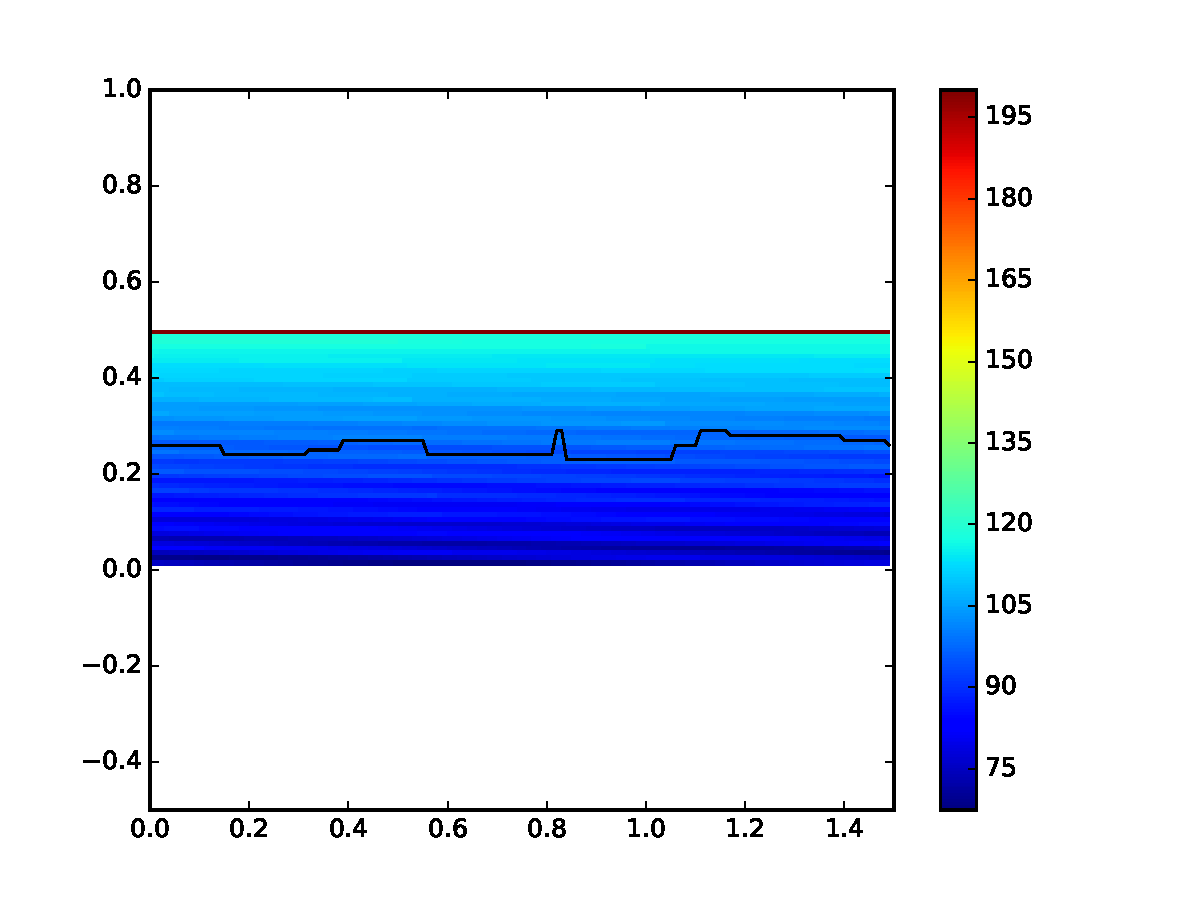
\includegraphics[scale=0.8]{Pseudocolor plot.pdf}
    \caption{An example of a pseudo color plot with an isoline
    to represent the location of the mean temperature}
    \label{fig:my_label}
\end{figure}

\begin{thebibliography}{2}
\bibitem{CME211Part2}
CME 211: Project Part 2 (Handout)
, Andreas Santucci, December 2021. Stanford
 CA.
\bibitem{CME211Part1}
CME 211: Project Part 1 (Handout)
, Andreas Santucci, November 2021. Stanford
 CA.

\end{thebibliography}

\end{document}
